\section{Постановка задачи}

Рассматривается двумерная задача Дирихле для уравнения Пуассона.
Требуется найти функцию $u(x,y)$, которая удовлетворяет уравнению внутри заданной области и принимает известные значения на её границе:
\begin{equation}
    -\Delta u=1 \quad \text{в }
    D, \qquad u=\sin(x+y) \quad \text{на } \gamma=\partial D.
    \label{eq:problem}
\end{equation}
Здесь $\Delta u=\partial^2u/\partial x^2+\partial^2u/\partial y^2$ есть оператор Лапласа, $D$ обозначает область расчёта, а $\gamma$ её границу.
Координаты и значения функции в задании безразмерны.

Варианту 14 соответствует область~\cite{assignment}
\begin{equation}
    D=\left\{(x,y):x^2+(|y|-2)^2<9\right\}.
    \label{eq:domain}
\end{equation}
Она представляет собой объединение двух кругов радиуса $3$ с центрами $(0,2)$ и $(0,-2)$.
Для вычислений выбран прямоугольник $\Pi=(-4,4)\times(-6,6)$, внутри которого целиком находится замыкание $D$.
Форма области и пример её распределения между процессами показаны на рис.~\ref{fig:geometry}.

\begin{figure}[ht]
    \centering
    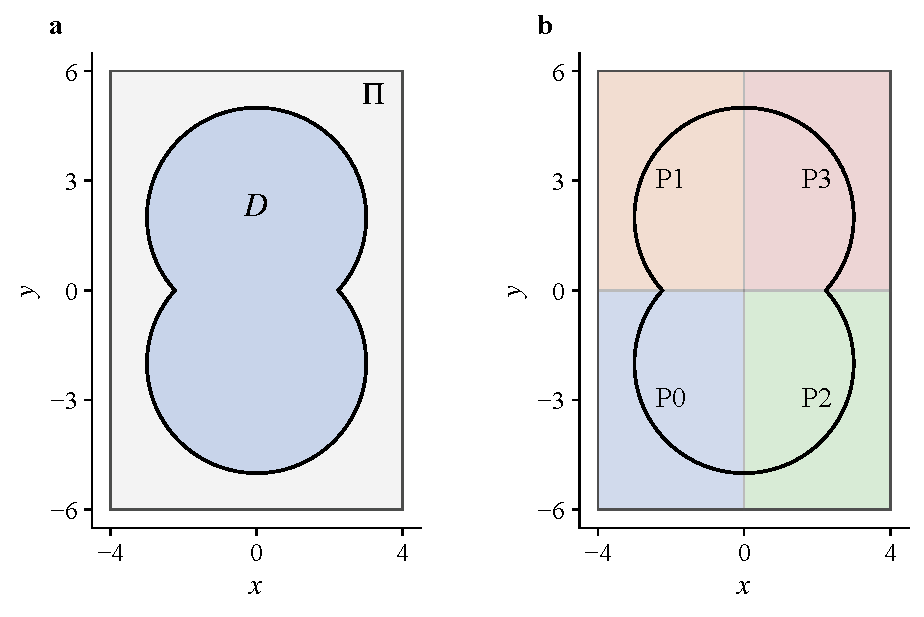
\includegraphics[width=0.94\linewidth]{figures/geometry.pdf}
    \caption{Расчётная геометрия: \textbf{a} область $D$ внутри прямоугольника $\Pi$; \textbf{b} пример разбиения $\Pi$ между четырьмя MPI-процессами. Цвет обозначает принадлежность геометрической подобласти процессу; граница исходной области показана чёрной линией.}
    \label{fig:geometry}
\end{figure}

Программа вычисляет приближённые значения $u$ в узлах сетки.
Для одной и той же схемы реализованы последовательный алгоритм, версия OpenMP, версия MPI и гибридная версия MPI+OpenMP.
Сравниваются полученные решения, число итераций и время вычислений.

\section{Метод фиктивных областей}

Прямоугольная сетка позволяет использовать одинаковый шаблон вычислений во всех узлах.
Для учёта криволинейной границы за пределами $D$ в уравнение вводится штрафной член, который приближает решение к заданному продолжению граничной функции.
В качестве продолжения выбрана функция $g(x,y)=\sin(x+y)$.
Задача в прямоугольнике имеет вид
\begin{equation}
    -\Delta v+Q(x,y)(v-g)=F(x,y) \quad \text{в }\Pi,
    \qquad v=g \quad \text{на }\partial\Pi,
    \label{eq:penalty}
\end{equation}
где
\begin{equation}
    Q(x,y)=\begin{cases}0,&(x,y)\in D,\\ \varepsilon^{-2},&(x,y)\in\Pi\setminus D,\end{cases}
    \qquad
    F(x,y)=\begin{cases}1,&(x,y)\in D,\\0,&(x,y)\in\Pi\setminus D.\end{cases}
    \label{eq:coefficients}
\end{equation}
При малом $\varepsilon$ член $Q(v-g)$ ограничивает отклонение $v$ от $g$ в фиктивной области.
Внутри $D$ сохраняется исходное уравнение Пуассона.
Согласно условию задания, используется $\varepsilon=h^2$, где $h$ есть наибольший шаг сетки~\cite{assignment}.
Такой выбор параметра сам по себе не задаёт точность конечного сеточного решения.
